\section{Автономний процес і надійність}
\subsection{Що саме автоматизує контролер}
Оркестратор інциденту приймає типізовану специфікацію інциденту, фіксовані входи аудиту Source Watch і бюджети ресурсів. У режимі виконання його реєстр у коді може викликати наявний вебзбирач із дозволеного переліку. Початкові URL не розширюють автоматично цей реєстр або перелік дозволених доменів. Нові маніфести збору можуть проходити через міст імпорту до локального для запуску реєстру доказів. Після цього можуть оброблятися необов'язкові типізовані офлайн-входи. Планування без виконання, виконання збору й локальний аналіз є явними незалежними опціями.

Офлайн-запускач викликає лінії походження, пошук, типізоване впорядкування часової шкали, інформаційні підсумки, надані входи конфлікту, сценарії невизначеності та перевірки звіту, якщо є сумісні входи. Відсутні входи він фіксує як заблоковані або не запущені, а не вигадує їх. Пошук не викликає евристик прийняття кураторського збирача тверджень. Формування звіту очікує окремо наданий набір із висновками, записами доказів і результатами перевірки. Тому успішне виконання контролера не свідчить, що сирі джерела автономно перетворено на перевірені висновки. Вирішальну межу показано на рисунку~\ref{fig:workflow}.

\begin{figure}[!htbp]
\centering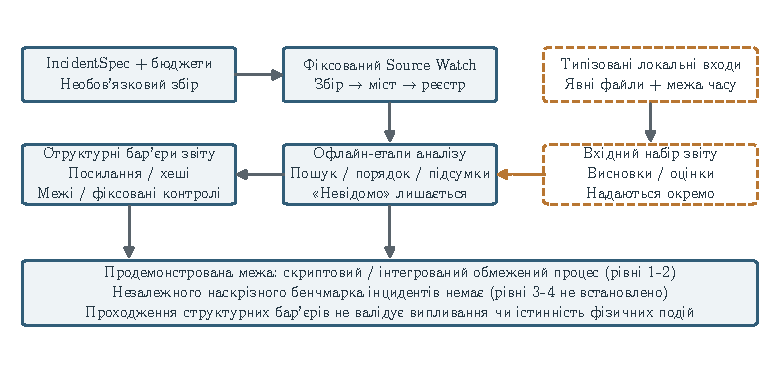
\includegraphics[width=\linewidth]{analysis_workflow.pdf}
\caption{Обмежений процес і межі автоматизації. Типізовані входи, кураторські судження й окремо запущений аналіз медіа надходять через явні інтерфейси. Структурні бар'єри можуть відхилити недійсні посилання, але не можуть перетворити кандидатний уривок на семантично обґрунтований висновок. Твердження про наскрізне розслідування лишається невалідованим.}
\label{fig:workflow}
\end{figure}

\subsection{Явна описова шкала автономності}
У цій статті рівень~0 означає ручну роботу; рівень~1 --- скриптову обробку наданих входів; рівень~2 --- інтегрований автоматизований аналітичний процес; рівень~3 --- автономний пошук і оцінку з урахуванням доказів у межах незалежно валідованих завдань; рівень~4 --- незалежно валідований наскрізний аналіз інцидентів із початково невідомими результатами. Це авторська описова шкала, а не стандарт спільноти чи порядкова міра точності.

Більшість збирачів, локальне індексування й кураторські збирачі працюють на рівні~1. Типізований офлайн-запускач і обмежений оркестратор демонструють інтеграцію рівня~2. Їхні семантичні входи й висновки лишаються обмеженими наданими даними та невиміряною якістю висновування. Окремо виконаний евристичний збирач тверджень не підносить усю систему до рівня~3; жоден поточний результат не демонструє рівень~4. Людські або зовнішньо валідовані еталонні набори потрібні під час розробки й оцінювання, але це не означає, що людина має розмічати кожен майбутній запис під час експлуатації. Натомість непідтримувані завдання мають лишатися невідомими або поза межами валідованої робочої області.

\subsection{Контрольні бар'єри надійності та невизначеність}
Оцінювальний каркас перевіряє форму схем, посилання, граничні часи, залежності джерел, хеші артефактів звіту й зафіксовані синтетичні сценарії. Семантичне оцінювання він явно позначає як невиконане. Зокрема, 783 пройдені тести не можуть означати 100\% фактичної точності. Структурне походження прийняття, як-от \code{validated_rule}, не встановлює, що правило було незалежно валідоване. Фіксовані значення евристичної впевненості не є каліброваними ймовірностями.

Сценарії невизначеності показують залежність від спірних міток, невідомих груп каналів, припущень про вилучення й обмеження та сконцентрованих спостережень. Їхні інтервали є сценарними межами, обумовленими наданими записами, а не вибірковими довірчими інтервалами для суспільної думки. Інкрементний запуск і порівняння звітів можуть виявляти зачеплені результати та змінені рішення, але не гарантують істинності переглянутого змістового висновку. Інженерним пріоритетом є прозорий збій і придатність для перегляду, що узгоджується з практиками відтворюваних досліджень \citep{sandve2013reproducible,wilson2017practices}; семантична надійність лишається окремим емпіричним завданням.
